\documentclass{beamer}
\usetheme{default}
\useoutertheme{infolines}
\setbeamertemplate{navigation symbols}{}

\usepackage{amsmath}
\usepackage{tikz}
\usetikzlibrary{arrows}

\usepackage[absolute,overlay]{textpos}
\newenvironment{reference}[2]{%
  \begin{textblock*}{\textwidth}(#1,#2)
      \footnotesize\it\bgroup\color{red!50!black}}{\egroup\end{textblock*}}

\newcommand{\D}{\mathcal{D}}
\newcommand{\ly}{\hat{y}(x;\D)}
\newcommand{\xt}{\tilde{x}}
\newcommand{\yt}{\tilde{y}}

% predefined font sizes:
% \tiny, \scriptsize, \footnotesize, \small, \normalsize (default),
% \large, \Large, \LARGE, \huge, \Huge
\begin{document}

\title{Active Learning with Statistical Models}
\subtitle{D. A. Cohn, Z. Ghahramani, M. I. Jordan}

\institute[]{Hauptseminar Machine Learning (WS 13/14)\\
Steffen Fuchs}
\author[S. Fuchs]{}

\date[15.01.2014]{January 15, 2014}

%%%_____________________________________________________________________________
%%%
%%%  title
%%%_____________________________________________________________________________
\begin{frame}[plain]
  \titlepage
\end{frame}

%%%_____________________________________________________________________________
%%%
%%%  overview
%%%_____________________________________________________________________________
\begin{frame}{Overview}
\begin{itemize}
  \item What is Active Learning?
  \item Active Learning - A Statistical Approach
  \item Example 1 - Gaussian Mixture Model
  \item Example 2 - Locally Weighted Regression
  \item Experimental Results
\end{itemize}
\end{frame}

%%%_____________________________________________________________________________
%%%
%%%  intro
%%%_____________________________________________________________________________
\begin{frame}{Introduction}
What is Active Learning and why would we need it?
\begin{itemize}
  \item Most of the time learners are treated as passive recipients of data
  \item In many situations a learner also has the ability to act, to gather data
    and to influence the world it is trying to understand
  \item Active learning is the study of how to use this ability effectively
\end{itemize}

\begin{center}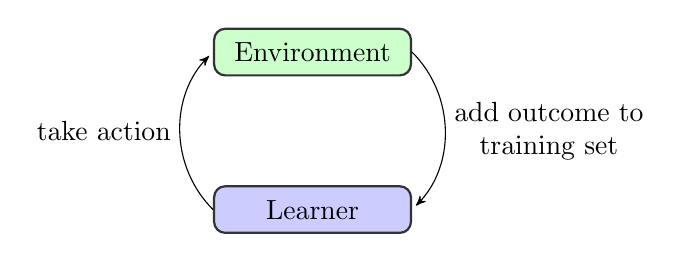
\begin{tikzpicture}[
  box/.style={rectangle,rounded corners,draw=black!80,thick,
    inner sep=5pt, minimum width=2.5cm, node distance=2cm},
  to/.style={->, >=stealth', shorten >=2pt},
  every node/.style={align=center}]

  \node[box,fill=green!20] (env) {Environment};
  \node[box,fill=blue!20] (mod)[below of=env] {Learner};

  \path (mod.west)
        edge[to,bend left=45] node[left]{take action} (env.west);
  \path (env.east)
        edge[to,bend left=45] node[right]{add outcome to \\ training set} (mod.east);
  %\draw (env) -- node[right]{add outcome to training set} -- (mod);
\end{tikzpicture}\end{center}
\end{frame}

%..............................................................................
\begin{frame}{Introduction}
Active learning offers its greatest rewards when
\begin{itemize}
  \item data is expensive or difficult to obtain
  \item the environment is complex or dangerous
\end{itemize}
Examples include
\begin{itemize}
  \item query human experts for labeling (natural language understanding,
    biomedical information extraction)
  \item selecting locations for sensor measurments to locate buried hazardous wastes
  \item selecting joint angles or torques to learn kinematics or dynamcis of a robot
\end{itemize}
\end{frame}

%%%_____________________________________________________________________________
%%%
%%%  GENERAL
%%%_____________________________________________________________________________
\begin{frame}{Active Learning - A Statistical Approach}
We define
\begin{itemize}
\item $P(x,y)$ as the unknown joint distribution
\item $P(x)$ the known marginal distribution of input $x$ and
\item $\ly$ as the learner's output for $x$, given training set $\D$
\end{itemize}
The expected error of the learner can be written as
\begin{equation}
    \int_x E_T \left[\left(\ly - y(x)\right)^2|x\right] P(x)dx
\end{equation}
where $E_T\left[ \cdot \right]$ denotes the expectation over $P(y|x)$ and $\D$.
\end{frame}

%..............................................................................
\begin{frame}{Active Learning - A Statistical Approach}
\begin{reference}{4mm}{85mm}
  S. Geman, E. Bienenstock and R. Doursat,
  Neural networks and the bias/variance dilemma, Neural computation 1992
\end{reference}

This expecation can be decomposed as
\small \begin{align}
    E_T \left[\left(\ly - y(x)\right)^2|x\right] =
    & \; E\left[\left(y(x) - E\left[y|x\right]\right)^2\right] \tag{2.1}\\
    & + \left( E_{\D} \left[\ly\right] - E\left[y|x\right]\right)^2 \tag{2.2}\\
    & + E_{\D} \left[\left(\ly - E_{\D} \left[\ly\right]\right)^2 \right] \tag{2.3}
\end{align}\normalsize
where
\begin{columns}[t]
\begin{column}{0.02\textwidth} \end{column} %empty
\begin{column}{0.98\textwidth}\begin{itemize}
  \item[{\small(2.1)}] is the variance of the distribution, not depending on the learner
  \item[{\small(2.2)}] is the squared bias of the learner(here: assumed to be zero)
  \item[{\small(2.3)}] is the learner's variance
\end{itemize}\end{column}
\end{columns}
\end{frame}

%..............................................................................
\begin{frame}{Active Learning - A Statistical Approach}
Thus, in order to minimize the learner's error, the only part we are interested
in is its variance
\begin{equation}\begin{split}
  \sigma_{\hat{y}}^2
  & = E_{\D} \left[\left(\ly - E_{\D} \left[\ly\right]\right)^2 \right] \\
  & = \left<(\hat{y} - \left<\hat{y}\right> )^2\right>
\end{split}\end{equation}
depending on $x$ and $\D$, where $\left< \cdot \right>$ denotes
$E_\D\left[\cdot\right]$.\\

For a new query at $\xt$, the resulting $(\xt,\yt)$ is added to $\D$, which
changes the expectation of the learner's variance
\begin{equation}
  \left< \tilde{\sigma}_{\hat{y}}^2 \right> =
  E_{\D\cup(\xt,\yt)} \left[\sigma_{\hat{y}}^2 | \xt \right]
\end{equation}
\end{frame}

%..............................................................................
\begin{frame}{Active Learning - A Statistical Approach}
The goal is to select data in a way to minimize the value of the
learner's variance intergraded over X.
\end{frame}

%%%_____________________________________________________________________________
%%%
%%%  Gaussian Mixture Model
%%%_____________________________________________________________________________

\begin{frame}{Gaussian Mixture Model (GMM)}
!!!IMAGE!!!
\begin{equation}
P(x,y|i) = \frac{1}{2\pi\sqrt{|\Sigma_i|}} \exp
\left[ -\frac{1}{2}(\mathbf{x}-\mu_i)^T\Sigma_i^{-1}(\mathbf{x}-\mu_i) \right]
\end{equation}
with
\[
\mathbf{x} = \left[ \begin{array}{c} x \\ y \end{array} \right] \quad
\mu_i = \left[ \begin{array}{c} \mu_{x,i} \\ \mu_{x,i} \end{array} \right] \quad
\Sigma_i = \left[ \begin{array}{cc} \sigma^2_{x,i} & \sigma_{xy,i} \\
    \sigma_{xy,i} & \sigma^2_{y,i} \end{array} \right] \quad
\]
obtained from an EM algorithm.
\end{frame}

\begin{frame}{Gaussian Mixture Model (GMM)}
By using these parameters one can compute the conditional expectation $\hat{y}$
and its variance as
\begin{equation}
  \hat{y} = ,\quad \sigma_{\hat{y}}^2 =
\end{equation}
where
\begin{equation}
n_i, \quad h_i, \quad P(x|i)
\end{equation}
just put all equations here!
\end{frame}


%%%_____________________________________________________________________________
%%%
%%%  Locally weighted regression
%%%_____________________________________________________________________________

\begin{frame}{Locally Weighted Regression (LWR)}

\end{frame}

\end{document}